\documentclass[a4paper,11pt,portuguese]{article}
\usepackage{geometry}
\usepackage{hyperref}
\usepackage{listings}
\usepackage{xcolor}
\usepackage{graphicx}
\usepackage{float}
\usepackage[portuguese]{babel}

\geometry{margin=0.9in}

%%% Estilo de código %%%

\definecolor{codegreen}{rgb}{0,0.6,0}
\definecolor{codegray}{rgb}{0.5,0.5,0.5}
\definecolor{codepurple}{rgb}{0.58,0,0.82}
\definecolor{backcolour}{rgb}{0.95,0.95,0.92}

\lstdefinestyle{mystyle}{
    backgroundcolor=\color{backcolour},   
    commentstyle=\color{codegreen},
    keywordstyle=\color{magenta},
    numberstyle=\tiny\color{codegray},
    stringstyle=\color{codepurple},
    basicstyle=\ttfamily\footnotesize,
    breakatwhitespace=false,         
    breaklines=true,                 
    captionpos=b,                    
    keepspaces=true,                 
    numbers=left,                    
    numbersep=5pt,                  
    showspaces=false,                
    showstringspaces=false,
    showtabs=false,                  
    tabsize=2
}

\lstset{style=mystyle}


\begin{document}

%%% Identificação %%%

\author{
    Diogo Costa\\
    \href{mailto:up201906731@edu.fe.up.pt}{up201906731@edu.fe.up.pt}
    \and
    Francisco Colino\\
    \href{mailto:up201905405@edu.fe.up.pt}{up201905405@edu.fe.up.pt}
}
\title{FEUP -- Redes de Computadores \large 2021/2022 \\ \large 1.º Trabalho Laboratorial}
\date{\today}
\maketitle

%%% Sumário %%%
\begin{center}
    \textbf{Sumário}
\end{center}

Este projeto foi realizado como sendo o 1.º projeto laboratorial da unidade curricular
\textit{Redes de Computadores}, fazendo esta parte da \textit{Licenciatura em Engenharia
Informática e Computação} da \textit{FEUP}. O projeto consistiu na implementação de um
protocolo de ligação de dados que permite a transferência confiável de dados entre dois
computadores através da porta série. Para além deste protocolo foi implementada uma
aplicação de transferência de ficheiros que faz uso do serviço fornecido pelo protocolo
de ligação de dados. \par

Todos os objetivos foram atingidos na medida em que foi implementado com sucesso um
protocolo de ligação de dados confiável e a aplicação que faz uso desse protocolo. Esta
implementação foi testada em contexto laboratorial e provou ser resistente a interrupções
e interferências. Foi ainda feita uma análise estatística experimental e comparados os
resultados aos expectados teoricamente.


%%% Introdução %%%
\section{Introdução}

    O objetivo deste trabalho é implementar um protocolo de ligação de dados, 
    de acordo com o guião fornecido, que permite fazer a transmissão de ficheiros 
    de forma assíncrona através de portas série assegurando a integridade dos ficheiros.
    Esta integridade deve ser assegurada mesmo com interrupções e interferências. 
    Este relatório procura expor a teoria por de trás deste projeto, como é que os
    objetivos foram alcançados e os testes efetuados à eficiência do protocolo. \par

    \hfill \break
    \noindent Este relatório está estruturado da seguinte forma:
    \begin{itemize}
        \item \textbf{Arquitetura} -- Blocos funcionais e interfaces.
        
        \item \textbf{Estrutura do Código} -- Demonstração das \textit{APIs}, principais 
        estruturas de dados, principais funções e a sua relação com a arquitetura.

        \item \textbf{Casos de uso principais} -- Identificação dos casos de uso 
        e representação das sequências de chamada de funções.

        \item \textbf{Protocolo de ligação lógica} -- Identificação dos principais
        aspetos funcionais da ligação lógica e descrição das estratégias usadas na
        implementação destes aspetos com extratos de código.

        \item \textbf{Protocolo de aplicação} -- Identificação dos principais
        aspetos funcionais da aplicação e descrição das estratégias usadas na
        implementação destes aspetos com extratos de código.

        \item \textbf{Validação} -- Descrição dos testes efetuados com apresentação
        quantificada dos resultados.

        \item \textbf{Eficiência do protocolo de dados} -- Caraterização estatística 
        da eficiência do protocolo, efetuada recorrendo a medidas sobre o código
        desenvolvido.

        \item \textbf{Conclusão} -- Síntese da informação apresentada nas secções
        anteriores e reflexão sobre os objetivos de aprendizagem alcançados.
        
    \end{itemize}


%%% Arquitetura %%%
\section{Arquitetura}
    
    O projeto está dividido em dois blocos funcionais principais, \textbf{\textit{Data Link}} e 
    \textbf{\textit{Application}}, podendo desempenhar dois papeis distintos, emissor e recetor.
    Estas duas camadas são independentes com o intuito de tornar o código mais modular de 
    modo a que a camada mais baixa possa ser usada com outras aplicações. \par
    
    A \textbf{camada de ligação de dados \textit{(Data Link)}} é o nível mais baixo. Esta trabalha
    com a porta série e oferece uma interface, que permite a abertura, fecho, leitura e escrita
    numa porta série. Esta permite comunicação assíncrona e fidedigna entre dois
    computadores com a capacidade de deteção e tratamento apropriado de erros, interrupções 
    e interferências sem que haja perdas de dados ou transferência de dados incorretos. \par 

    A \textbf{camada da aplicação \textit{(Application)}} é uma interface que usa a linha de
    comandos para comunicar com o utilizador. Esta oferece dois serviços: emissor e recetor.
    Em ambos, o utilizador tem a liberdade de escolher a porta série a utilizar e, no caso do emissor, 
    escolher o ficheiro a enviar e que nome dar a este no envio ao recetor. A aplicação é também
    responsável pela divisão do ficheiro original em pacotes de um tamanho predefinido para
    envio na camada de ligação de dados. \par 


%%% Estrutura do código %%%
\section{Estrutura do código}

    O código encontra-se dividido em 4 ficheiros \textit{.c} de modo a facilitar a divisão
    nas camadas mencionadas. \par
    
    Ao \textbf{\textit{Data Link}} corresponde o ficheiro \textit{linklayer.c}, à
    \textbf{\textit{Application}} correspondem os ficheiros \textit{aplic.c},
    \textit{receiver.c} e \textit{sender.c}.
    
    \hfill \break
    \noindent Funções principais da camada \textbf{\textit{Data Link}}:
    \begin{itemize}
        \item llopen() -- estabelece a ligação entre as máquinas através de tramas de Supervisão (S)
        \item llwrite() -- envia tramas de Informação (I) e recebe tramas de Supervisão (S)
        \item llread() -- lê tramas de Informação (I) e envia tramas de Supervisão (S)
        \item llclose() -- termina a ligação entre as máquinas através de tramas de Supervisão (S)
    \end{itemize}

    \hfill \break
    \noindent Macros principais da camada \textbf{\textit{Data Link}}:
    \begin{itemize}
        \item BAUDRATE -- valor da \textit{baud rate} a ser utilizada na comunicação
        \item TIME\_OUT\_TIME -- segundos que as funções esperam pelo 
        envio de dados antes de entrarem em \textit{timeout}
        \item MAX\_NO\_TIMEOUT -- número máximo de \textit{timeouts} consecutivos
        \item DATA\_PACKET\_MAX\_SIZE -- tamanho máximo que os dados do campo de informação,
        antes de \textit{stuffing}, podem ter por envio de pacote
    \end{itemize}

    \hfill \break
    \noindent Funções principais da camada \textbf{\textit{Application}}:
    \begin{itemize}
        \item send\_file() -- reparte um ficheiro em pacotes de tamanho predefinido e faz uso da função 
        llwrite() para os enviar
        \item receive\_file() -- recebe diversos pacotes de dados, fazendo uso da função llread(), 
        e organiza-os de forma a montar o ficheiro recebido
    \end{itemize}
    
    \hfill \break
    \noindent Macros principais da camada \textbf{\textit{Application}}:
    \begin{itemize}
        \item CONTROL\_PACKET\_MAX\_SIZE -- tamanho máximo de um pacote de controlo da aplicação
        \item PACKET\_MAX\_SIZE -- tamanho máximo de um pacote da aplicação, obtido como sendo
        o máximo entre o CONTROL\_PACKET\_MAX\_SIZE e o DATA\_PACKET\_MAX\_SIZE
        \item FILE\_NAME\_MAX\_SIZE -- tamanho máximo do nome de um ficheiro em \textit{linux}
    \end{itemize}

%%% Casos de uso principais %%%
\section{Casos de uso principais}

    \subsection{Transmissor}
    
        A aplicação é executada em modo \textbf{\textit{sender}}. O utilizador escolhe a porta série a
        utilizar, o caminho do ficheiro a mandar ao recetor e o nome que deve ser dado ao ficheiro
        na sua receção. Primeiro é estabelecida a ligação entre o transmissor e o recetor, verificando
        que o ficheiro passado à aplicação é válido este é então enviado em pacotes através duma porta
        série fazendo uso do mecanismo \textit{Stop-and-Wait}. Após o envio a ligação é terminada.
        Exemplo: \hfill \break
        ./sender 0 ``pinguim.gif'' ``p1.gif''

        \hfill \break
        \noindent Uma sequência mais detalhada do que acontece:
        \begin{enumerate}
            \item Abre a porta série e estabelece a conexão com fd = llopen(``/dev/ttyS0'', TRANSMITTER)
            \item Envia pacotes de controlo e o ficheiro repartido em pacotes de dados através da função llwrite()
            \item Fecha a porta série, terminando assim a ligação, com llclose()
        \end{enumerate}

    \subsection{Recetor}

        A aplicação é executada em modo \textbf{\textit{receiver}}. O utilizador escolhe a porta série a
        utilizar. Primeiro é estabelecida a ligação entre o transmissor e o recetor e é feita a leitura
        pacote a pacote do ficheiro a ser recebido. Após a leitura a ligação é terminada. Exemplo: \hfill \break
        ./receiver 4

        \hfill \break
        \noindent Uma sequência mais detalhada do que acontece:
        \begin{enumerate}
            \item Abre a porta série e estabelece a conexão com fd = llopen(``/dev/ttyS4'', RECEIVER)
            \item Os pacotes enviados pelo transmissor são lidos sequencialmente através da função llread()
            \item Fecha a porta série, terminando assim a ligação, com llclose()
        \end{enumerate}


%%% Protocolo de ligação lógica %%%
\section{Protocolo de ligação lógica}

    O protocolo de ligação lógica teve como objetivo fornecer um serviço de comunicação fiável entre
    dois sistemas ligados por um meio de comunicação, neste caso um cabo série. Este é responsável
    por algumas funcionalidades genéricas:
    \begin{itemize}
        \item Sincronismo de trama -- dados organizados em tramas
        \item Estabelecimento e encerramento da ligação
        \item Byte stuffing das informações das tramas assegurando transparência
        \item Transmissão de tramas
        \item Receção das trams com envio de resposta
        \item Controlo de erros
        \item Controlo de fluxo
    \end{itemize}
    
    \subsection{Estabelecimento da ligação}

    Para este efeito, o protocolo quando utilizado como transmitter envia uma trama de Supervisão (S) 
    com o seguinte formato, sendo que C terá valor de SET.

    \begin{itemize}
        \item F -- Flag
        \item A -- Campo de Endereço
        \item C -- Campo de Controlo:
            \begin{itemize}
                \item SET -- set up
                \item DISC -- disconnect
                \item UA -- unnumbered acknowledgment
                \item RR -- receiver ready
                \item REJ -- reject 
            \end{itemize}
        \item $BCC_1$ -- Campo de Proteção (cabeçalho) 
        \item F -- Flag
    \end{itemize}

    No lado do receiver ao receber uma trama (S) com C = SET, manda uma outra trama (S) mas com c = UA,
    funcionando como resposta de ACK. Para a construção destas tramas é usada a função:
    
\begin{lstlisting}[language=C]
static void control_frame_builder(control_frame_type_t cft, uint8_t msg[]);    
\end{lstlisting}

    O transmitter tem incorporado um timeout que ao enviar a trama espera pela resposta de receiver. Se
    ao fim de 3 segundos não obtiver resposta, reenvia a trama. Este processo é repetido 3 vezes sendo que
    o programa termina no 3º timeout. Se a receção da trama (S) com C = UA for feita com sucesso pelo transmitter, então a ligação é dada
    como estabelecida. Todo este processo é realizado pela função:

\begin{lstlisting}[language=C]
int llopen(int porta, type_t type);    
\end{lstlisting}

    \subsection{Envio de tramas}

    Depois da confirmação de que a ligação foi estabelecida, pode-se começar a enviar tramas de
    informação. Os pacotes a serem enviados, através destas tramas, serão referidos como P. As tramas de 
    informação têm o seguinte formato:

    \begin{itemize}
        \item F -- flag
        \item A -- Campo de Endereço
        \item C -- Campo de Controlo:
        \item $BCC_1$ -- Campo de Proteção (cabeçalho)
        \item $D_1...D_n$ -- Campo de informação (contém pacote gerado pela aplicação)
        \item $BCC_2$ -- Campo de Proteção (dados)
        \item F -- flag
    \end{itemize}

    O $BCC_2$ é calculado através da aplicação da operação XOR entre todos os bytes do pacote P, 
    um \textit{foldright} com a operação XOR. Isto é feito através da função:

\begin{lstlisting}[language=C]
uint8_t bcc2_builder(uint8_t msg[], unsigned int msg_size);    
\end{lstlisting}

    Após a construção do $BCC_2$ procede-se a fazer stuffing do pacote P, resultando no
    campo $D_1...D_n$, e do próprio $BCC_2$. Esta operação é importante porque assegura a transparência.

    Agora reunem-se as condições para enviar a trama. Após o envio desta, o transmitter fica à espera
    de uma mensagem de resposta do receiver que será uma trama (S) com C = RR se o receiver aceitar a
    trama e quiser a próxima e C = REJ se o receiver rejeitar a trama e precisar que o transmitter a
    reenvie.

    O transmitter tem incorporado um timeout que ao enviar a trama espera pela resposta de receiver. Se
    ao fim de 3 segundos não obtiver resposta, reenvia a trama. Este processo é repetido 3 vezes sendo que
    o programa termina no 3º timeout.

\begin{lstlisting}[language=C]
int llwrite(int fd, uint8_t *buffer, int length);   
\end{lstlisting}

    \subsection{Receção de tramas}

    O receiver fica à espera de que lhe sejam enviadas tramas de informação (I) no formato referido
    anteriormente, e à medida que vai recebendo dados vai validando-os através de uma máquina de estados.

    Alguns comportamentos importantes a salientar são os comportamentos na receção dos BCC.
    No caso de erro de $BCC_1$ o receiver descarta todos os dados dessa trama e não envia resposta, o que
    leva o transmitter a dar time-out e a reenviar a trama.

    Após a receção de todos os dados, que é detetada com a recção da Flag final, o campo de informação 
    + $BCC_2$ são \textit{destuffed} e a partir do campo de informação é computado um segundo $BCC_2$.

    \noindent Na comparação do $BCC_2$ recebido com o computado:
    \begin{itemize}
        \item Inválido
            \begin{itemize}
                \item Se não for uma trama duplicada é enviado REJ
                \item Se for duplicada, não são guardados os dados e é enviado RR
            \end{itemize}
        \item Válido
            \begin{itemize}
                \item Se não for uma trama duplicada, são guardados os dados e é enviado RR
                \item Se for duplicada, não são guardados os dados e é enviado RR
            \end{itemize}
    \end{itemize}

    \noindent De notar que as mensagens de REJ e RR são montadas com o valor de R=N(r) que depois é
    usado para comparação com o valor S=N(s) recebido pelo campo C das tramas de Informação,
    influenciando as validações do cabeçalho.

\begin{lstlisting}[language=C]
int llread(int fd, uint8_t *buffer);
\end{lstlisting}

    \subsection{Terminação da ligação}

    Para encerrar a ligação, o transmitter manda uma trama de (S) com C = DISC, o receiver quando
    recebe DISC manda ele próprio um DISC e o transmitter por fim manda UA, sinalizando assim
    a terminação correta da ligação. Estas operações também estão protegidas por time-outs similares
    aos mencionados anteriormente.

\begin{lstlisting}[language=C]
int llclose(int fd, type_t type);
\end{lstlisting}


%%% Protocolo de aplicação %%%
\section{Protocolo de aplicação}

    O protocolo de aplicação implementado teve como objetivo a tranferência de um ficheiro fazendo uso
    da interface fornecida pela camada de ligação lógica. O protocolo implementado tem as seguintes
    características:

    \subsection{Tipos de pacotes}
    A aplicação faz uso de dois tipos de pacotes: pacotes de dados, usados para transferir pedaços de ficheiro,
    e pacotes de controlo, usados para sinalizar o início e fim de uma transferência.
    
    \noindent A seguinte função definida em
    \textit{aplic.c} monta um pacote de controlo:

\begin{lstlisting}[language=C]
static uint8_t* get_control_packet(off_t file_size, char *file_name, int file_name_size, int *length);
\end{lstlisting}

    Nesta função, é gerado o pacote de controlo START. Ela recebe como parâmetros o tamanho e o nome
    do ficheiro e retorna um pointer para um pacote de controlo assim como um retorno por parâmetro
    do tamanho desse pacote. O pacote de controlo tem a seguinte composição:

    \begin{itemize}
        \item C -- 1 byte de campo de controlo (2: START; 3: END)
        \item TLV (Type, Length, Value) -- os necessários, neste caso 2 (tamanho e nome de ficheiro)
            \begin{itemize}
                \item T -- 1 byte que indica o tipo de parâmetro (0: tamanho de ficheiro; 1: nome do ficheiro)
                \item L -- 1 byte que indica o tamanho do campo seguinte, V
                \item V -- valor do parâmetro que ocupa o número de bytes indicado em L
            \end{itemize}
    \end{itemize}

    \hfill \break
    \noindent Por outro lado, os pacotes de dados têm a seguinte composição:

    \begin{itemize} \label{pacotesdados}
        \item C -- 1 byte de controlo (1: DADOS)
        \item N -- 1 byte de número de sequência em módulo 255
        \item $L_2L_1$ -- 2 bytes com o número de bytes (K) do campo de dados
        \item $P_1...P_k$ -- K bytes de dados
    \end{itemize}

    \hfill \break
    \noindent Estes pacotes são montados e enviados na seguinte função definida em \textit{aplic.c}:

\begin{lstlisting}[language=C]
static int send_packaged_file(int fd_serial_port, int fd_file);
\end{lstlisting}


    \subsection{Envio de ficheiro}
    O envio de um ficheiro é efetuado recorrendo à seguinte função:

\begin{lstlisting}[language=C]
int send_file(int porta, char *path, int path_size, char *file_name);
\end{lstlisting}

    \noindent Esta abre o ficheiro a enviar e abre uma conexão usando \textit{llopen()}, da camada
    de ligação lógica, na porta série que recebeu como argumento. De seguida, envia o pacote de controlo
    START, previamente montado, usando \textit{llwrite()}. Após isso torna-se necessário enviar o
    ficheiro repartido por vários pacotes de dados. Para tal, recorre-se à seguinte função já referida
    anteriormente:

\begin{lstlisting}[language=C]
static int send_packaged_file(int fd_serial_port, int fd_file);
\end{lstlisting}

    \noindent Ela vai enviando os pacotes usando \textit{llwrite()} à medida que lê pedaços de ficheiro usando
    \textit{read()}. Nestes pacotes, como já referido na secção \hyperref[pacotesdados]{Tipos de pacotes}, 
    vão também outras informações. \par
    
    Após o ficheiro ser enviado na totalidade, é então enviado o pacote de controlo END e após isso, basta fechar 
    a conexão usando \textit{llclose()} e fechar o ficheiro aberto usando \textit{close()}.

    
    \subsection{Receção de ficheiro}
    A receção de um ficheiro é efetuado recorrendo à seguinte função:
    
\begin{lstlisting}[language=C]
int receive_file(int porta);
\end{lstlisting}
    
    \noindent Esta função começa por abrir uma conexão na porta série usando \textit{llopen()}
    e de seguida vai começar a ler pacotes usando \textit{llread()}.

    Numa execução ela começará por receber o pacote de controlo START. Após isto, já sabe o nome do ficheiro
    e o tamanho do mesmo. Com esta informação cria um ficheiro e abre-o em modo \textit{append}.
    De seguida vai recebendo pacotes de dados dos quais retira as porções de ficheiro e acrescenta-as ao
    final do ficheiro criado anteriormente. No final, irá receber um pacote de controlo END e saberá
    que a transmissão chegou ao fim podendo fechar o ficheiro usando \textit{close()} e a conexão da porta série
    usando \textit{llclose()}.


%%% Validação %%%
\section{Validação}

    De modo a validar o correto funcionamento dos protocolos de ligação de dados
    e de aplicação foram efetuados múltiplos testes, tanto em ambiente simulado usando
    o utilitário da linha de comandos \textit{socat} e o ficheiro de exemplo fornecido,
    \textit{cable.c}, como em ambiente laboratorial no laboratório I321 na
    \textit{FEUP}. Em ambiente laboratorial foi testado o envio de diversos ficheiro
    de 4 modos distintos:

    \begin{itemize}
        \item Sem interrupções e sem interferências.
        \item Com interrupções mas sem interferências.
        \item Sem interrupções mas com interferências.
        \item Com interrupções e com interferências.
    \end{itemize}

    Em todas as situações, os protocolos provaram ser robustos uma vez que garantiram o
    correto envio sem erros dos ficheiros enviados. Esta certeza foi garantida através do
    uso do utilitário da linha de comandos \textit{diff} que foi utilizado para comparar
    na máquina recetora o ficheiro recebido com uma cópia que a mesma já tinha do ficheiro. \par

    Foi também testada a ordem de execução dos programas: \textit{receiver} seguido pelo
    \textit{sender} e \textit{sender} seguido pelo \textit{receiver} obtendo
    em ambas as situações um correto funcionamento do envio de ficheiros.

%%% Eficiência do protocolo de ligação de dados %%%
\section{Eficiência do protocolo de ligação de dados}

    De forma a avaliar a eficiência do protocolo de ligação de dados implementado, foi efetuada
    uma caracterização estatística da eficiência (S) em função de a e do \textit{FER}
    (Frame error ratio). Os valores resultantes foram então comparados com valores teóricos. \hfill \break
    Os valores que deram origem aos gráficos que se seguem podem ser lidos em anexo.

    \subsection{S = f(a)}
    De modo a variar experimentalmente o valor de \textit{a}, foi variado o valor de $T_{prop}$
    introduzindo um ligeiro atrasado usando \textit{usleep()}. Isto é possível dado que
    $a = T_{prop}/T_f$. Foi obtido o seguinte gráfico que mostra que os valores medidos seguem a
    tendência teórica:

    \begin{figure}[H]
        \centering
        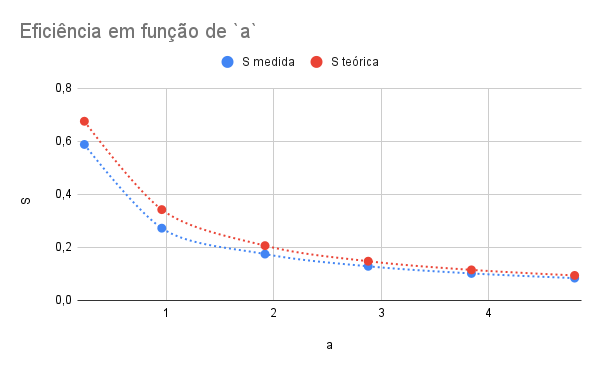
\includegraphics[scale=0.5]{./imgs/a.png}
        \caption{Eficiência em função de a.}
        \label{fig:a}
    \end{figure}


    \subsection{S = g(FER)}
    De modo a variar experimentalmente o valor de FER foram introduzidos erros fictícios nos
    $BCC_1$ e $BCC_2$ de acordo com o FER pretendido e obteve-se o seguinte gráfico que mostra
    que os valores medidos seguem a tendência teórica:

    \begin{figure}[H]
        \centering
        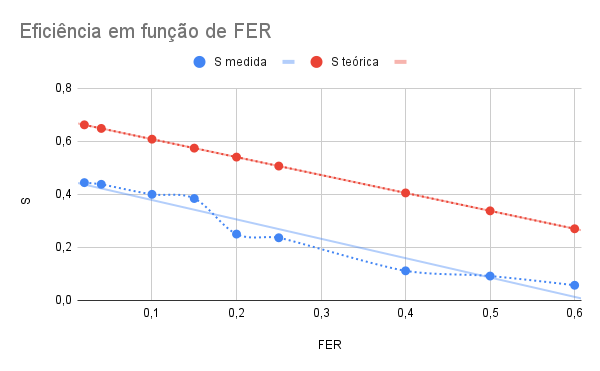
\includegraphics[scale=0.5]{./imgs/fer.png}
        \caption{Eficiência em função de FER.}
        \label{fig:fer}
    \end{figure}


%%% Conclusões %%%
\section{Conclusões}

    Foram implementados em C dois protocolos robustos, ligação de dados e aplicação, para
    transferir ficheiros entre computadores usando a porta série. Foi garantida
    independência entre camadas e a correta implementação do mecanismo de
    \textit{Stop-and-Wait} para controlo de erros no protocolo de ligação
    de dados. Foi ainda escrito este relatório que inclui uma análise de eficiência.
    Assim, foram cumpridos todos os objetivos deste projeto. \par

    A realização deste projeto permitiu lidar na prática com os detalhes abordados
    teoricamente nas aulas que de outra forma nos passariam despercebidos. Assim sendo,
    a sua conceção demonstrou ser uma forma de estudo imersiva dos conteúdos lecionados
    em \textit{Redes de Computadores}.


%%% Anexos %%%
\newpage

\section{Anexos}
\subsection{Código Fonte}

\lstinputlisting[language=C, caption=sender.c]{../src/sender.c}

\lstinputlisting[language=C, caption=receiver.c]{../src/receiver.c}

\lstinputlisting[language=C, caption=aplic.h]{../src/aplic.h}

\lstinputlisting[language=C, caption=linklayer.h]{../src/linklayer.h}

\lstinputlisting[language=C, caption=aplic.c]{../src/aplic.c}

\lstinputlisting[language=C, caption=linklayer.c]{../src/linklayer.c}


\subsection{Eficiência em função de 'a'}
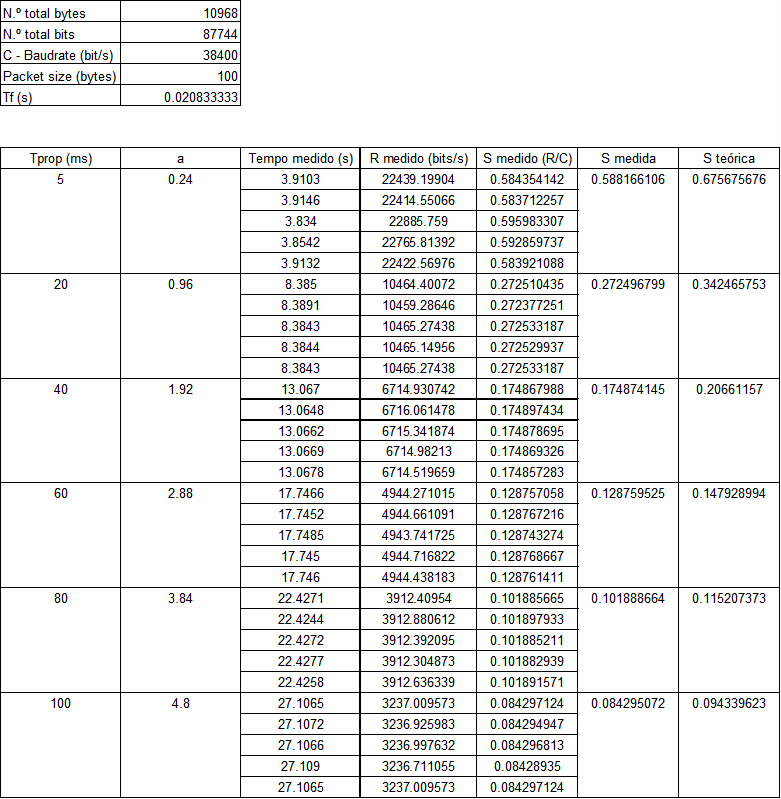
\includegraphics[scale=0.6]{./imgs/grapha.png}


\subsection{Eficiência em função de FER}
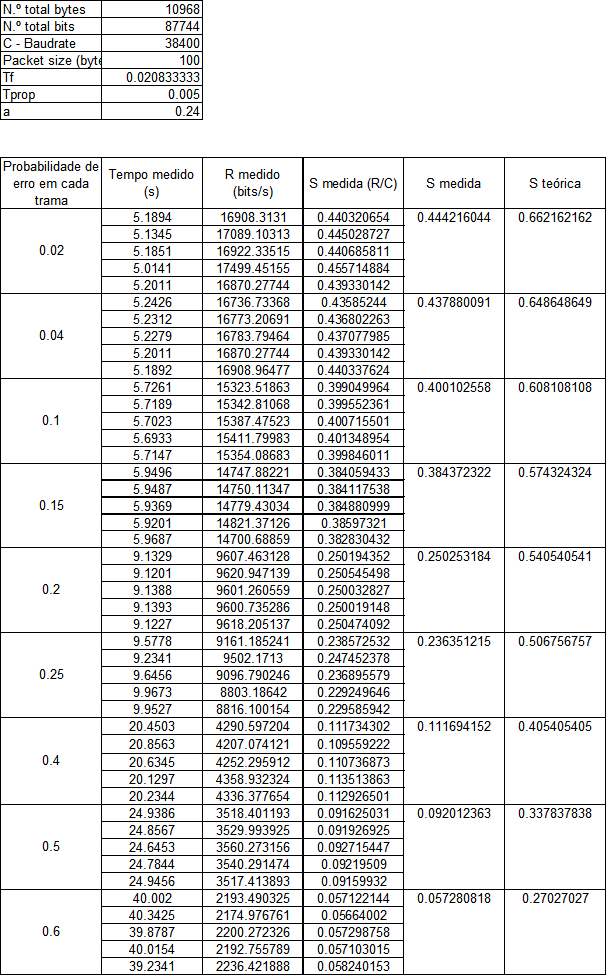
\includegraphics[scale=0.8]{./imgs/graphfer.png}

\end{document}
